\section{Overall Description}\label{sec overall-desc}

\subsection{Product Perspective}
PowerEnJoy system is a simple client-server architecture based on a back-end server application and diffent front-end client applications, supported by different operating systems.

\subsubsection{User Interfaces}
Guests and users can interact with the service via the web application or the mobile application. Drivers can find other service functionalities in the car application. It is necessary to provide a common and uniform look and feel among the different hardware architectures.

All the interfaces shall be intuitive and user friendly. They should not require the reading of detailed documentation to be used.

\subsubsection{Hardware Interfaces}

The main hardware interface is a dedicated embedded system, installed in any vehicles, provided of several plugins and a touchscreen display for interact with the car application.
Thanks to this embedded architecture the system will be also notified about the status of the vehicle and its location, even if the main battery is completely discharged.

\subsubsection{Software Interfaces}
Mobile application and web application are supposed to be friendly with any device, in particular the first one must be developed for iOS and Android, and the second one will work on any operating system that support a web browser.

On the embedded system of any vehicles is installed a JVM that runs a Java application that provides informations to the driver and to the system.

The back-end server stores its data in a RDBMS and can run on every platform that supports the JVM. It also provides different APIs for different functions that a user, or a guest, can do through client applications. 

\subsection{Product Functions}
\begin{figure}[H]
	\centering
	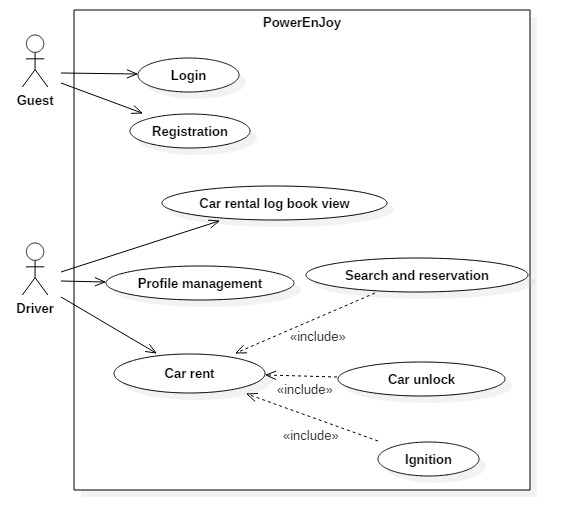
\includegraphics[width=\textwidth]{use_cases/PowerEnJoy.jpg}
	\caption{The comprehensive use-case diagram of all the functionalities implemented by the system.}
\end{figure}

\begin{figure}[H]
	\centering
	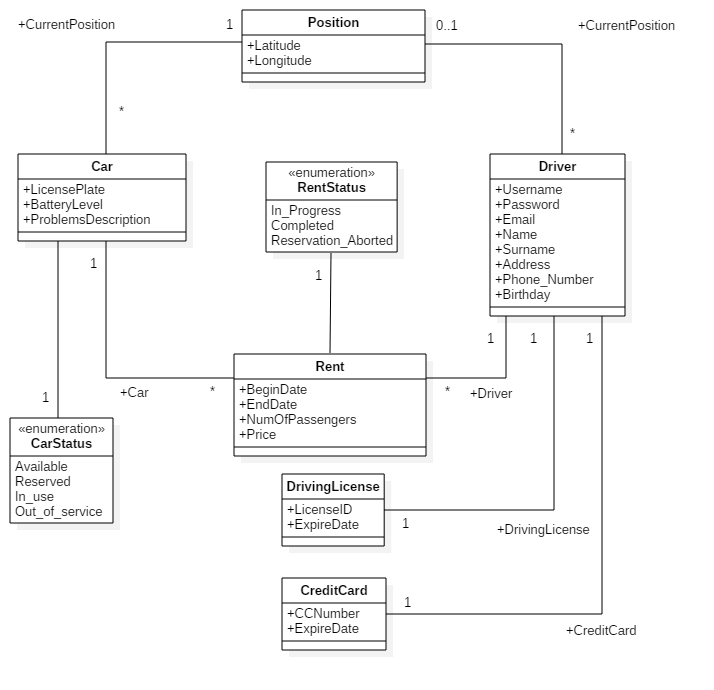
\includegraphics[width=\textwidth]{uml/PowerEnJoy.jpg}
	\caption{The comprehensive class diagram of the system.}
\end{figure}

The following lists reassume what anyone can do interacting with the system.
\begin{itemize}
	\item Guests can:
	\begin{itemize}
		\item create an account (signup to the system)
		\item login
	\end{itemize}
	\item Drivers can:
	\begin{itemize}
		\item edit profile informations
		\item delete their account
		\item rent a vehicle
		\item check their status
		\item access to the vehicle rental log book
	\end{itemize}
	\item Operators can:
	\begin{itemize}
		\item solve vehicle problems
	\end{itemize}
\end{itemize}

\subsection{User Characteristics}
The two kinds of users are drivers and operators. Only drivers can registered to the system independently, while operators must obtain a contract of employment with the PowerEnJoy service to access as operators. The system provides special accounts for them and they would be able to access to their job functionalities through the same, web and mobile applications, of drivers. They will be recognized by the system and a special view will be provided to them.

It's granted that both kinds of users have access to Internet.

\subsection{Constraints}

\subsubsection{Regulatory policies}
Any driver must follow current traffic and regulamentation laws of the area where the system is operating its car-sharing service. Driving licenses from other countries must be compatible with the laws of the country where the service is operating.
Aggiungere regolamentazioni di lavoro

\subsubsection{Service policies}
\begin{itemize}
	\item The system must ask the user for the permission to acquire, store and process personal data and web cookies.
	\item A driving license can't be associated to multiple driver accounts.
	\item Drivers with status of pending payments can't delete their accounts and can't access to rental functions.
	\item Drivers with invalid/expired driving license can't access to rental functions
	\item Drivers can rent a single vehicle per time.
\end{itemize}	

\subsubsection{Hardware limitations}
The service requires an Internet connection fast enought to guarantee a fast response from the server and hardware architectures that can run properly the client side applications (web and mobile apps).

\subsubsection{Reliability requirements}
The system must have a minimum availability of 98\%.

\subsubsection{Parallel operations}
The system must support parallel operations from different drivers that may require access to the database.

\subsection{Assumptions and Dependencies}

It assumes that:
\begin{itemize}
	\item All users have access to a stable Internet connection.
	\item All drivers have a valid credit card.
	\item The GPS on the vehicle is working correctly.
	\item The driver specifies the correct location, if its GPS is not available.
	\item Vehicles model is the same, so any cars will have the same number of seats.
	\item Vehicle's sensors can detect correctly the number of passengers.
	\item The System applies a correct discount at the end of the renting and than charges the drivers directly via credit card.
	\item The System provides to make a vehicle available again if will pass more than one hour from the reservation time.
	\item The number of vehicles is sufficient to satisfy the demand in each area.
	\item Any fine taken by a driver will be paid by the system that will charge him/her for the same fine plus an additional fine provided by the system.
	\item All the areas where the system is operating are covered by a reliable 3G/4G connection.
	\item Operators are arranged in convenient locations that allow them to be efficient and fast when recovering and charging vehicles.
	\item The system is operating in an area composed by a city or agglomerated cities, of the same country, closed each other.
	\item The application on the vehicle will automatically notify the system about incidents, vehicle failures or low charges. If the application will stop to dialogate with the server, the system will considered it like a notification of vehicle failure in the last position assumed by the vehicle.
\end{itemize}

\subsection{Future Extensions}
The system will be implemented foreseeing the possibility of further extensions, for example:

\begin{enumerate}
	\item If a vehicle is left at special parking areas where they can be recharged and the driver take care of pluggin the vehicle into the power grid, the system applies a discount of 30\% on the last ride.
	\item If a vehicle is left at more than 3 KM from the nearest power grid station or with more than 80\% of the battery empty, the system charges 30\% more on the last ride to compensate to compensate for the cost required to re-charge the vehicle on-site.
	\item If the driver enables the money saving option, he/she can input his/her final destination and the system provides information about the station where to leave the vehicle to get a discount. This station is determinate to ensure a uniform distribution of vehicles in the city and depends both on the destination of the driver and on the availability of power plugs at the selected station.
\end{enumerate}